\documentclass[nobib]{tufte-handout}

%\\geometry{showframe}% for debugging purposes -- displays the margins

\newcommand{\bra}[1]{\left(#1\right)}
\usepackage{amssymb}
\usepackage{hyperref}
\usepackage[activate={true,nocompatibility},final,tracking=true,kerning=true,spacing=true,factor=1100,stretch=10,shrink=10]{microtype}
\usepackage{color}
\usepackage{steinmetz}
% Fixes captions and images being cut off
\usepackage{marginfix}
\usepackage{array}
\usepackage{tikz}
\usepackage{amsmath,amsthm}
\usetikzlibrary{shapes}
\usetikzlibrary{positioning}
\usepackage{listings}
\usepackage{caption}
\usepackage{circuitikz}
\DeclareCaptionFont{white}{\color{white}}
\DeclareCaptionFormat{listing}{\colorbox{gray}{\parbox{\textwidth}{#1#2#3}}}
\captionsetup[lstlisting]{format=listing,labelfont=white,textfont=white}

% Set up the images/graphics package
\usepackage{graphicx}
\setkeys{Gin}{width=\linewidth,totalheight=\textheight,keepaspectratio}
\graphicspath{{.}}

\title{Notes for ECE 20002 - Electrical Engineering Fundamentals II}
\author[Shubham Saluja Kumar Agarwal]{Shubham Saluja Kumar Agarwal}
\date{\today}  % if the \date{} command is left out, the current date will be used

% The following package makes prettier tables.  We're all about the bling!
\usepackage{booktabs}

% The units package provides nice, non-stacked fractions and better spacing
% for units.
\usepackage{units}

% The fancyvrb package lets us customize the formatting of verbatim
% environments.  We use a slightly smaller font.
\usepackage{fancyvrb}
\fvset{fontsize=\normalsize}

% Small sections of multiple columns
\usepackage{multicol}

% For finite state machines 
\usetikzlibrary{automata} % Import library for drawing automata
\usetikzlibrary{positioning} % ...positioning nodes
\usetikzlibrary{arrows} % ...customizing arrows
\tikzset{node distance=2.5cm, % Minimum distance between two nodes. Change if necessary.
    every state/.style={ % Sets the properties for each state
    semithick,
    fill=gray!10},
    initial text={}, % No label on start arrow
    double distance=2pt, % Adjust appearance of accept states
    every edge/.style={ % Sets the properties for each transition
    draw,
    ->,>=stealth', % Makes edges directed with bold arrowheads
    auto,
    semithick}}
\let\epsilon\varepsilon

% These commands are used to pretty-print LaTeX commands
\newcommand{\doccmd}[1]{\texttt{\textbackslash#1}}% command name -- adds backslash automatically
\newcommand{\docopt}[1]{\ensuremath{\langle}\textrm{\textit{#1}}\ensuremath{\rangle}}% optional command argument
\newcommand{\docarg}[1]{\textrm{\textit{#1}}}% (required) command argument
\newenvironment{docspec}{\begin{quote}\noindent}{\end{quote}}% command specification environment
\newcommand{\docenv}[1]{\textsf{#1}}% environment name
\newcommand{\docpkg}[1]{\texttt{#1}}% package name
\newcommand{\doccls}[1]{\texttt{#1}}% document class name
\newcommand{\docclsopt}[1]{\texttt{#1}}% document class option name

% Define a custom command for definitions and biconditional
\newcommand{\defn}[2]{\noindent\textbf{#1}:\ #2}
\let\biconditional\leftrightarrow

\begin{document}

\maketitle

\begin{abstract}
These are lecture notes for spring 2024 ECE 20002 at Purdue. Modify, use, and distribute as you please.
\end{abstract}

\tableofcontents

\section{Course Introduction}

Continuation of Electrical and Computer Engineering Fundamentals I. The course addresses
mathematical and computational foundations of circuit analysis (differential equations, Laplace Transform techniques) with a focus on application to linear circuits having variable behavior as a function of frequency, with emphasis on filtering. Variable frequency behavior is considered for applications of electronic components through single-transistor and operational amplifiers. The course ends with a consideration of how circuits behave and may be modeled for analysis at high frequencies.\\
Learning Objectives:
\begin{enumerate}
    \item Analyze 2nd order linear circuits with sources and/or passive elements
    \item Compute responses of linear circuits with and without initial conditions via one-sided Laplace transform techniques
    \item Compute responses to linear circuits using transfer function and convolution techniques
    \item Analyze and design transistor amplifiers at low, mid and high frequencies
\end{enumerate}

\pagebreak 

\section{ECE 20001 Review}
Sinusoidal Signal (voltage and current) involve phasors, which bring complex numbers to the forefront. When in Sinusoidal Steady State (SSS):\\
\begin{equation*}
    Z_R=R
\end{equation*}
\begin{equation*}
    Z_L=j\omega L
\end{equation*}
\begin{equation*}
    Z_C=\frac{1}{j\omega C}
\end{equation*}
This can in turn be represented as as the following function:\\
\begin{equation*}
    x(t)=K_0 cos(\omega t + \theta_0)
\end{equation*}
Which can be transformed into the following form:\\
\begin{align*}
    K_0 e^{j(\omega t + \theta_0)} &= K_0 e^{j \theta_0}\\ 
    &= K_0 (cos(\theta_0) + j sin(\theta_0))\\ 
    &= K_0\phase{\theta_0}
\end{align*}
This can be represented as the following in the cartesian plane:\\
\begin{center}
    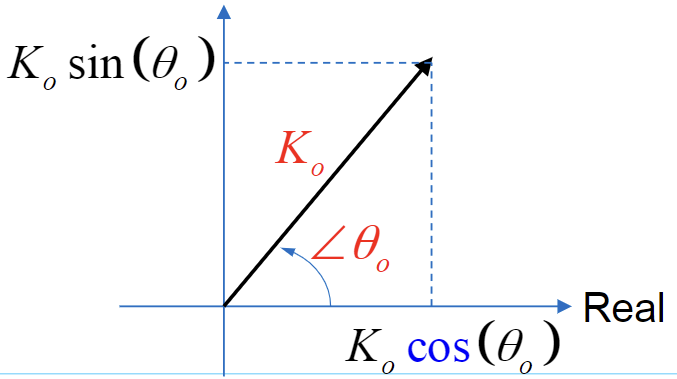
\includegraphics[width = 150px]{images/Screenshot 2024-01-08 155954.png}
\end{center}
Thus, these forms can be summed as following:\\
\begin{table}
 \centering
    \begin{tabular}{c|c}
    x(t) & $\mathbf{X}$\\
    \hline
    $K cos(\omega t)$ & K\\
    $K sin(\omega t) = K cos(\omega t)$ & $-Kj$\\
    $cos(\omega t) - sin(wt)$ & $1+j$\\
    $a cos(\omega t) + b sin(\omega t)$ & $a-bj$
    \end{tabular}
\end{table}
This is especially useful for circuit analysis methods such as KCL and KVL.
The methods of conversion between polar and phasor are:\\
\begin{equation*}
    z=a+bj
\end{equation*}
\begin{equation*}
    z=\rho \phase{\theta}
\end{equation*}
\begin{equation*}
    \rho = |z| = \sqrt{a^2 + b^2}
\end{equation*}
\begin{equation*}
    \theta = \text{phase(}z\text{)}=tan^{-1}(\frac{b}{a})
\end{equation*}
These conversions and operations alongside KCL and KVL, can allow us to create a system of differential equations that will allow us to solve almost any circuit. However, we don't like ODEs, so we have developed methods to get around this.\\
We know that at SSS, the following equations are valid.\\
\begin{center}
\begin{align*}
    V_R &= RI_R\\
    V_L &= j\omega LI_L\\
    V_C &= \frac{1}{j \omega C}I_C\\
    i_L(t) &= i_L(0) + \frac{1}{L} \int v_L \,dt\\
    V_C(t) &= V_C(0) + \frac{1}{C} \int i_C \,dt\\
\end{align*}

\end{center}
This can be used to solve most SSS circuits, using the aforementioned strategies, alongside strategies like current and voltage division.
Example:
\begin{center}
        \begin{circuitikz}[american currents]
        \draw (0,0)
        to[I, l=$I$] (0,2)
        to [short, -*] (1,2)
        to [L, l=$L$] (1,0)
        to [short, -] (0,0);
        \draw (1,2)
        to [short, -*] (2,2)
        to [R, l=$R$] (2,0)
        to [short, *-*] (1,0);
        \draw (2,2)
        to [short, -] (2.5,2);
        \draw (2,0)
        to [short, -] (2.5,0);
        \end{circuitikz}
\end{center}
\begin{align*}
    I_L=\frac{Z_L}{Z_R+Z_L}*I=\frac{j \omega L}{R+j \omega L}*I\\
    I_R=\frac{Z_R}{Z_R+Z_L}*I=\frac{R}{R+j \omega L}*I
\end{align*}
\pagebreak
\section{Using Ordinary Differential Equations to solve RL and RC circuits}
This section will provide a brief explanation of nonhomogenous differential equations and their applications to circuits.
\subsection{Ordinary Differential Equations (ODE) Overview}
Differential equations rely a lot on two properties. The invariablity of the exponential function across derivatives, and the ability to express any function in terms of the exponential function itself. That is,\\
\begin{equation*}
    e^t=\frac{d}{dt}e^t=\frac{d^2}{dt^2}e^t \cdots
\end{equation*}
Let us take the following differential equation as an example:
\begin{equation*}
    y(t)=6x(t)+3\frac{d}{dt}x(t)
\end{equation*}
We assume $x_h(t)=Ae^{\lambda t}$, and try to solve the homogenous equation $0=6x(t)+3x'(t)$.
\begin{align*}
    0 &= 6x+3x'\\
    0 &= 6Ae^{\lambda t} + 3A \lambda e^{\lambda t}\\
    0 &= 6+3\lambda\\
    \lambda &= -2\\
    \implies x_h(t) &= e^{-2t}
\end{align*}
At this point, we will consider two different cases: $y(t) = 4e^{3t}$ and $y(t) = 3e^{-2t}$.
We will find the particular solution $x_p(t)$ for each of these cases, as they have different methods of resolution.
\begin{align*}
    4e^{3t} &= 6x+3x'\\
    \text{Assume } x_p(t) &= Be^{3t}\\
    4e^{3t} &= 6Be^{3t} + 9Be^{3t}\\
    4 &= 15B\\
    B &= \frac{15}{4}\\
    \implies x_p(t) &= \frac{15}{4}e^{3t}\\
    \implies x(t) &= x_h(t)+x_p(t)=Ae^{-2t}+\frac{15}{4}e^{3t}
\end{align*}
Let us assume $y(0) = 4$
\begin{align*}
    \implies 4 &= A + \frac{15}{4}\\
    \implies A &= \frac{1}{4}\\
    \implies x(t) &= \frac{1}{4}e^{-2t}+\frac{15}{4}e^{3t}
\end{align*}
On the other hand, if $y(t) = 3e^{-2t}$, since $x_p(t)$ and $x_h(t)$ cannot have the same form, we will need to make a few changes:
\begin{align*}
    3e^{-2t} &= 6x+3x'\\
    \text{Assume } x_p(t) &= Bte^{-2t}\\
    3e^{-2t} &= 6Bte^{-2t} + 3Be^{-2t} - 6Bte^{-2t}\\
    \implies 3 &= 3B\\
    \implies B&=1\\
    \implies x_p(t) &= te^{-2t}
\end{align*}
Which can then be substituted into $x(t)$, allowing the differential equation to be fully solved by using the initial conditions.
\subsection{Using ODEs in circuits}
We will be solving the following two circuits:
\begin{center}
    \begin{circuitikz}[american voltages]
    \draw (0,2)
    to[V, l=$V_{in}$] (0,0);
    \draw (0,2)
    to [R, l=$R$] (2,2)
    to [L, l=$L$] (2,0)
    to [short, -] (0,0);
    \end{circuitikz}
    \begin{circuitikz}[american voltages]
    \draw (0,2)
    to[V, l=$V_{in}$] (0,0);
    \draw (0,2)
    to [R, l=$R$] (2,2)
    to [C, l=$C$] (2,0)
    to [short, -] (0,0);
    \end{circuitikz}
\end{center}
In the inductor circuit, if $i_L(0)=0$, we know:
\begin{align*}
    v_L &= L\frac{di_L(t)}{dt}\\
    v_L(t) &= v_{in}(t) - Ri_L(t)\\
    v_{in}(t) &= L\frac{di_L(t)}{dt} - Ri_L(t)
\end{align*}
By solving this equation as shown previously, we will find that $\lambda = -\frac{R}{L}$ which is in fact the inverse of the time constant for an RL circuit.
Under the assumption of $V_{in}$ being a constant, the particular solution will in fact be $i_p(t)=\frac{V_{in}}{R}=i_L(\infty)$. This results in the familiar equation:
\begin{equation*}
    i_L(t) = i_L(\infty) + (i_L(t_0)-i_L(\infty))e^{-\frac{R}{L}(t-t_0)}
\end{equation*} 
The same is done for the capacitor circuit, which ends up resulting in the once again familiar equation:
\begin{equation*}
    v_C(t) = v_C(\infty) + (v_C(t_0)-v_C(\infty))e^{-\frac{t-t_0}{RC}}
\end{equation*}
\end{document}